\documentclass[10pt,twocolumn,letterpaper]{article}

\usepackage{cvpr}
\usepackage{graphicx}
\usepackage{booktabs}
\usepackage{multirow}
\usepackage{makecell}
\usepackage{array}
\usepackage{amsmath}
\usepackage{amssymb}
\usepackage{adjustbox}
\usepackage{subcaption}
\usepackage{url}


\definecolor{cvprblue}{rgb}{0.21,0.49,0.74}
\usepackage[pagebackref,breaklinks,colorlinks,allcolors=cvprblue]{hyperref}

\def\paperID{AIAA3201}
\def\confName{CVPR}
\def\confYear{2026}

\title{Video Object Removal and Inpainting: From Hand-Crafted Baselines to Foundation-Model Pipelines\\
{\large AIAA3201 - Introduction to Computer Vision}\\
{\large Group Project Report}
}

\author{
  \normalfont Chi Kit WONG \\
  50012338\\
  \and
  Haodong XU \\
  50012601\\
}

\begin{document}
\maketitle

\begin{abstract}
This report studies automatic video object removal under the AIAA3201 project setting. We build three progressively stronger pipelines: a hand-crafted baseline that combines YOLOv8-Seg, sparse optical-flow motion filtering, temporal background propagation, and OpenCV inpainting; an AI-driven reproduction using SAM 2 or VGGT4D masks with ProPainter; and an exploration stage using SAM 3 masks with ProPainter, DiffuEraser, and ROSE inpainting backends. We evaluate mask quality on all 90 DAVIS validation sequences using Jaccard mean (JM) and Jaccard recall (JR), and evaluate video restoration on paired Wild Video clips using PSNR and SSIM. SAM 2 is a strong Part 2 baseline (JM 0.9167, JR 0.9846), while the SAM 3 multi-object setup improves DAVIS mask quality to JM 0.9423 and JR 0.9952. The best Wild Video PSNR is achieved by SAM 3 + DiffuEraser, while SAM 3 + ROSE-SE yields the best SSIM. GitHub repository: \url{https://github.com/Chikit-WONG/AIAA3201-Introduction_to_Computer_Vision-Project}.
\end{abstract}

\section{Introduction}
Video object removal requires two coupled capabilities: the system must identify the foreground object that should be removed, and it must synthesize a plausible background in the missing region. This is harder than single-image inpainting because masks must remain temporally stable and the filled background must avoid frame-to-frame flicker. The project therefore exposes the main tension in video restoration: segmentation errors propagate into inpainting artifacts, while inpainting models can still fail even when the mask is accurate if the hidden background is never visible.

We organize the work into three parts. Part 1 implements a classical pipeline from first principles. It uses YOLOv8-Seg detections, Lucas-Kanade optical flow to reject static detections, mask dilation, temporal background borrowing, and a Telea inpainting fallback. Part 2 reproduces stronger open-source systems by pairing SAM 2 or VGGT4D masks with ProPainter. Part 3 explores stronger mask and generative restoration choices: SAM 3 is used as the tracker, and ProPainter, DiffuEraser, and ROSE are compared as inpainting backends.

\section{Related Work}
Object detection and instance segmentation provide the front end for object removal. R-CNN introduced region-based CNN detection \cite{girshick2014rcnn}, while Mask R-CNN added a mask branch for instance segmentation \cite{he2017maskrcnn}. YOLO formulated detection as a single-stage real-time prediction problem \cite{redmon2016yolo}, and DETR later cast detection as direct set prediction with transformers \cite{carion2020detr}.

Recent foundation models shift segmentation from fixed-category detection to promptable object selection and tracking. SAM \cite{kirillov2023sam} provides promptable image segmentation, Track Anything combines SAM with video memory propagation \cite{yang2023trackanything}, SAM 2 extends the promptable formulation to video \cite{ravi2024sam2}, and SAM 3 introduces concept-level segmentation \cite{carion2025sam3}. VGGT and VGGT4D mine geometric and motion cues from visual geometry transformers \cite{wang2025vggt,hu2025vggt4d}; Pi3 and MapAnything are relevant newer geometry foundation models \cite{wang2025pi3,keetha2025mapanything}.

For video inpainting, FGVC uses flow-edge guidance for video completion \cite{gao2020fgvc}, E2FGVI proposes an end-to-end flow-guided framework \cite{li2022e2fgvi}, and ProPainter improves propagation and sparse-transformer inpainting \cite{zhou2023propainter}. Generative alternatives include latent diffusion models \cite{rombach2022ldm} and conditional control such as ControlNet \cite{zhang2023controlnet}, which motivate our Part 3 DiffuEraser and ROSE trials.

\section{Method}
\paragraph{Overall pipeline.}
Figure~\ref{fig:pipeline} summarizes the system. Each method follows the same high-level structure: extract frames, estimate or prompt object masks, optionally refine masks, inpaint the masked regions, and evaluate the outputs. The parts differ mainly in the mask source and inpainting backend.

% \begin{figure*}[t]
% \centering
% 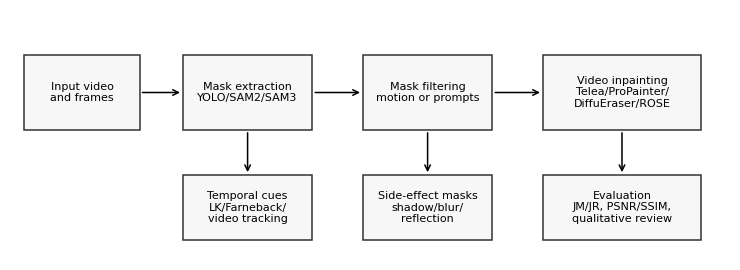
\includegraphics[width=0.96\linewidth]{figures/pipeline_flowchart_v1.png}
% \caption{Unified roadmap used across the three project parts. The same frame, mask, inpainting, and evaluation interfaces make the classical, reproduced, and exploratory pipelines directly comparable.}
% \label{fig:pipeline}
% \end{figure*}

\begin{figure*}[t]
\centering
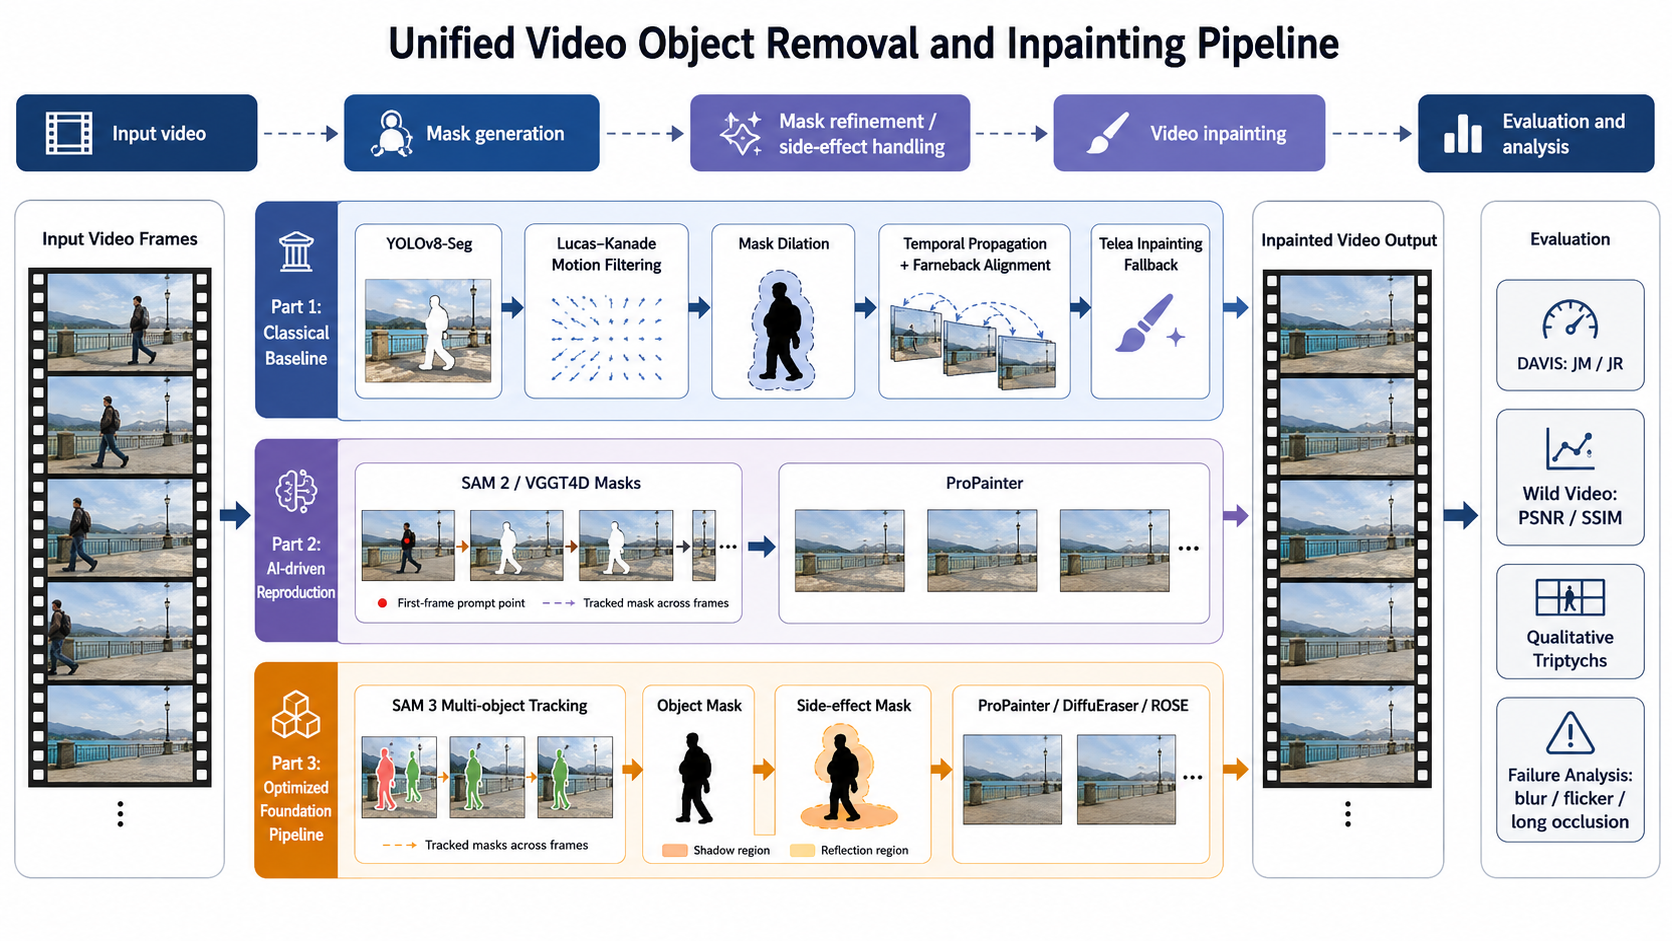
\includegraphics[width=0.96\linewidth]{figures/pipeline_flowchart_v2.png}
\caption{Unified roadmap used across the three project parts. The same frame, mask, inpainting, and evaluation interfaces make the classical, reproduced, and exploratory pipelines directly comparable.}
\label{fig:pipeline}
\end{figure*}

\paragraph{Part 1: hand-crafted baseline.}
The baseline extracts person masks with YOLOv8-Seg and then applies Lucas-Kanade sparse optical flow inside each instance mask. If the mean feature displacement is below a threshold, the object is treated as static and removed from the mask. We dilate accepted masks to cover motion blur and boundary uncertainty. For restoration, the temporal variant searches nearby frames in a sliding window. With optical-flow alignment enabled, neighboring frames and masks are warped into the current frame coordinate system using Farneback dense flow before clean pixels are copied. Remaining holes are filled by \texttt{cv2.inpaint} with Telea inpainting.

\paragraph{Part 2: AI-driven reproduction.}
Part 2 tests two mask sources with the same ProPainter backend. SAM 2 receives first-frame prompts and tracks objects through the video. VGGT4D is used as a training-free motion-cue baseline, but its dynamic masks are less aligned with the object-removal objective. ProPainter then propagates valid content and applies transformer-based completion, giving a stronger temporal inpainting model than the Part 1 spatial fallback.

\paragraph{Part 3: optimization and extension.}
Part 3 uses SAM 3 as the mask tracker and compares five restoration variants: ProPainter, DiffuEraser, DiffuEraser with side-effect masks, ROSE, and ROSE with side-effect masks. The side-effect mask expands the object mask, adds a shifted shadow region, and can include reflection regions for scenes where removing only the visible object leaves secondary traces. We also upgraded SAM 3 initialization to use per-object masks instead of a single union mask, matching the multi-object prompting pattern used by SAM 2. This change improves tracking stability on DAVIS.

\section{Experiments}
\paragraph{Datasets and metrics.}
We use the mandatory bmx-trees and tennis sample sequences, two paired Wild Video clips, and the full DAVIS validation set. DAVIS evaluation reports mask quality only: JM is mean IoU over frames and JR is the fraction of frames with IoU at least 0.5. For the Wild Video pair, clean no-person videos are available, so we report PSNR and SSIM against those clean references. Full-frame PSNR/SSIM on DAVIS would compare restored backgrounds against frames that still contain foreground objects, so it is not used for the formal DAVIS table.

\begin{table*}[t]
\centering
\small
\setlength{\tabcolsep}{4pt}
\caption{Mask quality on all 90 DAVIS validation sequences. Part 3 rows share the same SAM 3 masks, so JM/JR are identical across inpainting backends.}
\label{tab:davis-main}
\begin{tabular}{llccc}
\toprule
Part & Method & \#Seq. & JM $\uparrow$ & JR $\uparrow$ \\
\midrule
Part 1 & P1 spatial only & 90 & 0.2435 & 0.2355 \\
Part 1 & P1 temporal, no align & 90 & 0.2435 & 0.2355 \\
Part 1 & P1 temporal + flow & 90 & 0.2435 & 0.2355 \\
Part 2 & P2 VGGT4D + ProPainter & 90 & 0.1090 & 0.0269 \\
Part 2 & P2 SAM 2 + ProPainter & 90 & 0.9167 & 0.9846 \\
Part 3 & P3 SAM 3 + ProPainter & 90 & \textbf{0.9423} & \textbf{0.9952} \\
Part 3 & P3 SAM 3 + DiffuEraser & 90 & \textbf{0.9423} & \textbf{0.9952} \\
Part 3 & P3 SAM 3 + DiffuEraser-SE & 90 & \textbf{0.9423} & \textbf{0.9952} \\
Part 3 & P3 SAM 3 + ROSE & 90 & \textbf{0.9423} & \textbf{0.9952} \\
Part 3 & P3 SAM 3 + ROSE-SE & 90 & \textbf{0.9423} & \textbf{0.9952} \\
\bottomrule
\end{tabular}
\end{table*}

\begin{figure*}[t]
\centering
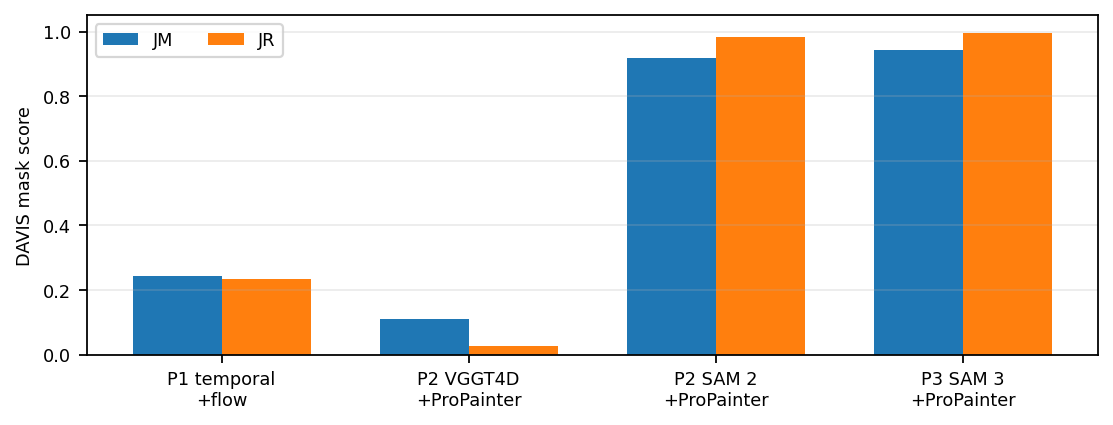
\includegraphics[width=0.95\linewidth]{figures/davis_mask_quality.png}
\caption{DAVIS average mask quality over all 90 validation sequences. SAM 2 is already strong, and the SAM 3 multi-object setup gives the best JM/JR among evaluated methods.}
\label{fig:davis-chart}
\end{figure*}

Table~\ref{tab:davis-main} shows that mask quality dominates the task. The Part 1 baseline is conservative but limited by category detections and classical motion filtering. VGGT4D performs poorly as a direct object-removal mask extractor because its motion cues do not reliably isolate the foreground instance. SAM 2 gives a large gain, and SAM 3 further improves the average to JM 0.9423 and JR 0.9952. Since all Part 3 backends reuse the same SAM 3 masks, their DAVIS JM/JR values are identical.

\begin{table}[t]
\centering
\scriptsize
\setlength{\tabcolsep}{3pt}
\caption{Representative DAVIS sequence-level mask metrics. The two course samples are bmx-trees and tennis; rhino is included because it exposes long-occlusion restoration failures.}
\label{tab:sample-metrics}
\begin{tabular}{llcc}
\toprule
Method & Seq. & JM $\uparrow$ & JR $\uparrow$ \\
\midrule
P1 temporal + flow & bmx-trees & 0.2671 & 0.0125 \\
P1 temporal + flow & tennis & 0.4922 & 0.4000 \\
P1 temporal + flow & rhino & 0.0000 & 0.0000 \\
P2 VGGT4D + ProPainter & bmx-trees & 0.0288 & 0.0000 \\
P2 VGGT4D + ProPainter & tennis & 0.0261 & 0.0000 \\
P2 VGGT4D + ProPainter & rhino & 0.0179 & 0.0000 \\
P2 SAM 2 + ProPainter & bmx-trees & 0.7399 & 0.9375 \\
P2 SAM 2 + ProPainter & tennis & 0.9362 & 1.0000 \\
P2 SAM 2 + ProPainter & rhino & 0.9808 & 1.0000 \\
P3 SAM 3 masks & bmx-trees & 0.7618 & 0.9500 \\
P3 SAM 3 masks & tennis & 0.9566 & 1.0000 \\
P3 SAM 3 masks & rhino & 0.9838 & 1.0000 \\
\bottomrule
\end{tabular}
\end{table}

\paragraph{Wild Video restoration.}
Table~\ref{tab:wild-main} and Figure~\ref{fig:wild-chart} summarize the paired Wild Video metrics. Part 2 SAM 2 + ProPainter improves over all Part 1 variants, confirming that better video masks and temporal inpainting matter. In Part 3, DiffuEraser gives the highest PSNR, while ROSE-SE gives the highest SSIM. These metrics are useful but not complete: PSNR favors pixel-level agreement, whereas temporal flicker and perceptual sharpness still require visual inspection.

\begin{table*}[t]
\centering
\small
\setlength{\tabcolsep}{4pt}
\caption{Wild Video quality against paired no-person clean videos. Values are averaged over Wild\_Video1 and Wild\_Video2.}
\label{tab:wild-main}
\begin{tabular}{llccc}
\toprule
Part & Method & \#Videos & PSNR $\uparrow$ & SSIM $\uparrow$ \\
\midrule
Part 1 & P1 temporal + flow & 2 & 13.6620 & 0.1737 \\
Part 1 & P1 temporal, no align & 2 & 13.6605 & 0.1736 \\
Part 1 & P1 spatial only & 2 & 13.6883 & 0.1749 \\
Part 2 & P2 SAM 2 + ProPainter & 2 & 14.3966 & 0.2002 \\
Part 2 & P2 VGGT4D + ProPainter & 2 & 12.9820 & 0.2057 \\
Part 3 & P3 SAM 3 + ProPainter & 2 & 13.6800 & 0.1902 \\
Part 3 & P3 SAM 3 + DiffuEraser & 2 & \textbf{14.4704} & 0.2289 \\
Part 3 & P3 SAM 3 + DiffuEraser-SE & 2 & 14.4680 & 0.2295 \\
Part 3 & P3 SAM 3 + ROSE & 2 & 14.2764 & 0.2319 \\
Part 3 & P3 SAM 3 + ROSE-SE & 2 & 14.4286 & \textbf{0.2323} \\
\bottomrule
\end{tabular}
\end{table*}

\begin{figure*}[t]
\centering
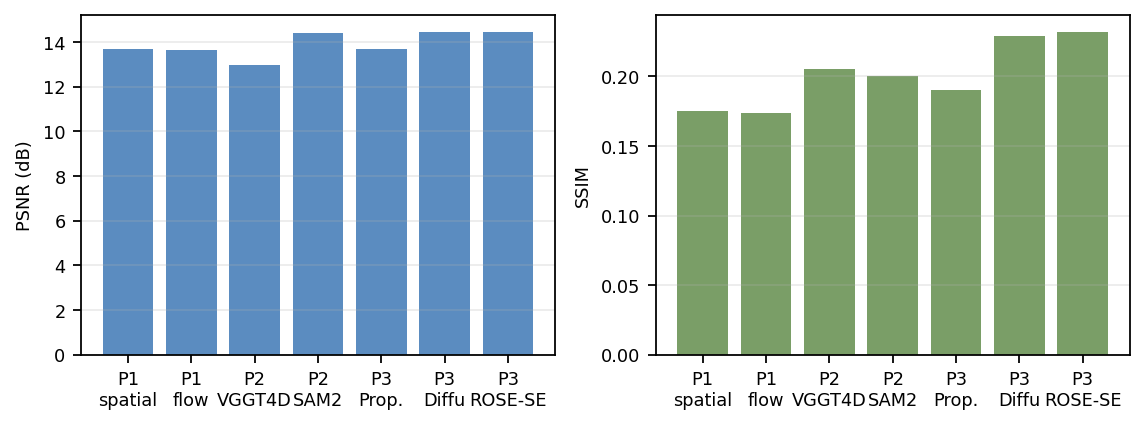
\includegraphics[width=0.95\linewidth]{figures/wild_video_quality.png}
\caption{Wild Video quality averaged over two paired clips. Part 3 generative backends improve SSIM, while DiffuEraser obtains the best PSNR among explored methods.}
\label{fig:wild-chart}
\end{figure*}

\begin{figure*}[t]
\centering
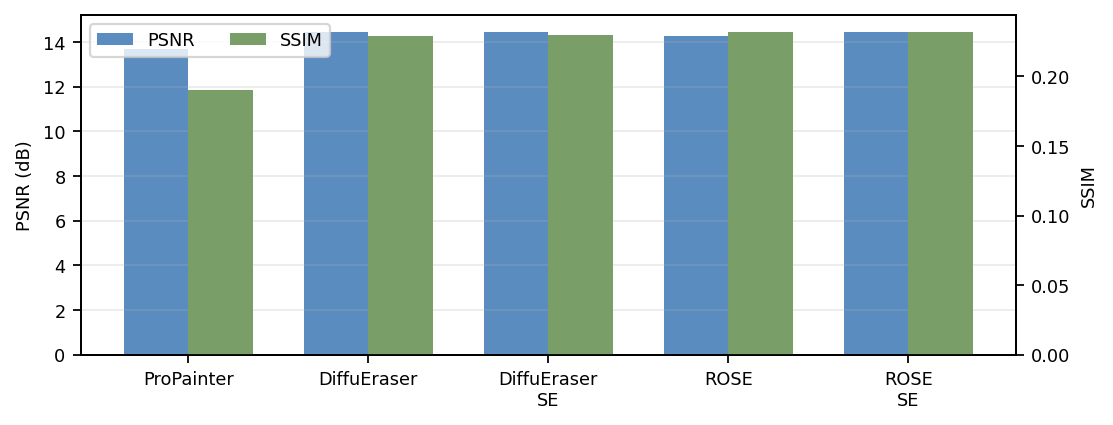
\includegraphics[width=0.95\linewidth]{figures/part3_backend_tradeoff.png}
\caption{Part 3 inpainting-backend trade-off on Wild Video. All rows use SAM 3 masks; only the restoration backend and side-effect mask choice change.}
\label{fig:part3-backends}
\end{figure*}

\paragraph{Qualitative comparison.}
Figures~\ref{fig:p1-qual}--\ref{fig:p3-qual} provide the required original-mask-inpaint triptychs for each part. All three figures use the same bmx-trees frame so that the visual differences come from the pipeline rather than from video content. The Part 1 result often preserves some foreground residue because the classical temporal borrowing step depends on mask accuracy and optical-flow alignment. Part 2 benefits from sharper SAM 2 masks and ProPainter's propagation. Part 3 uses SAM 3 masks and generative restoration, which can remove the object more completely but may smooth fine background texture.

\begin{figure}[t]
\centering
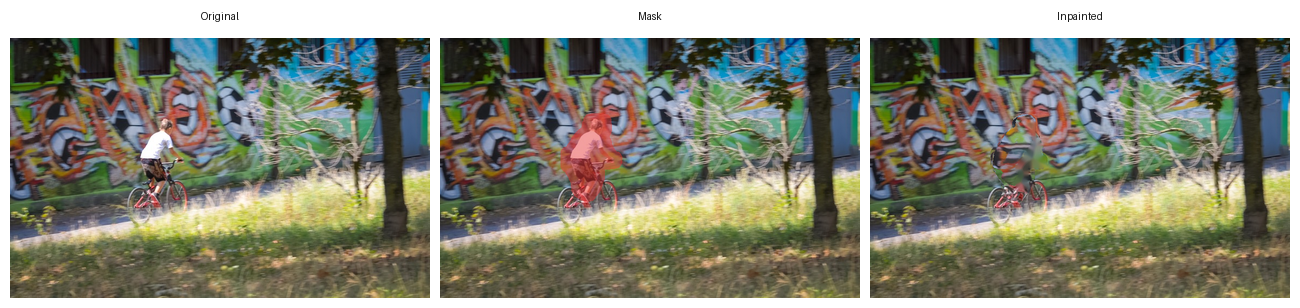
\includegraphics[width=\linewidth]{figures/part1_triptych.png}
\caption{Part 1 triptych on bmx-trees frame 30: original frame, YOLO/flow mask, and temporal-flow inpainting result.}
\label{fig:p1-qual}
\end{figure}

\begin{figure}[t]
\centering
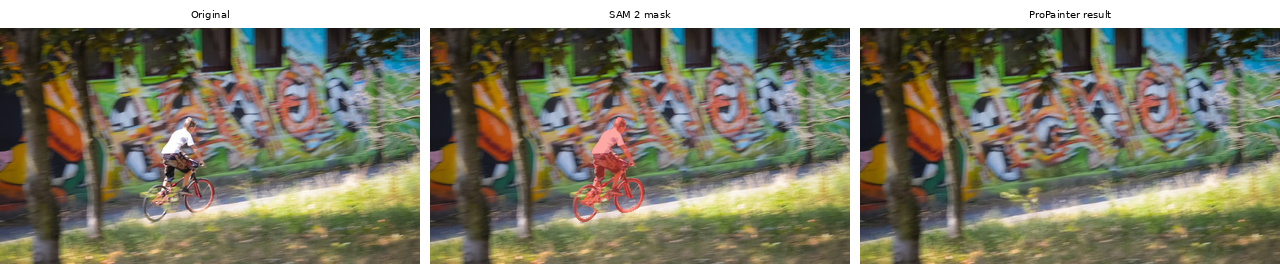
\includegraphics[width=\linewidth]{figures/part2_triptych.png}
\caption{Part 2 triptych on the same bmx-trees frame: original frame, SAM 2 mask, and ProPainter result.}
\label{fig:p2-qual}
\end{figure}

\begin{figure}[t]
\centering
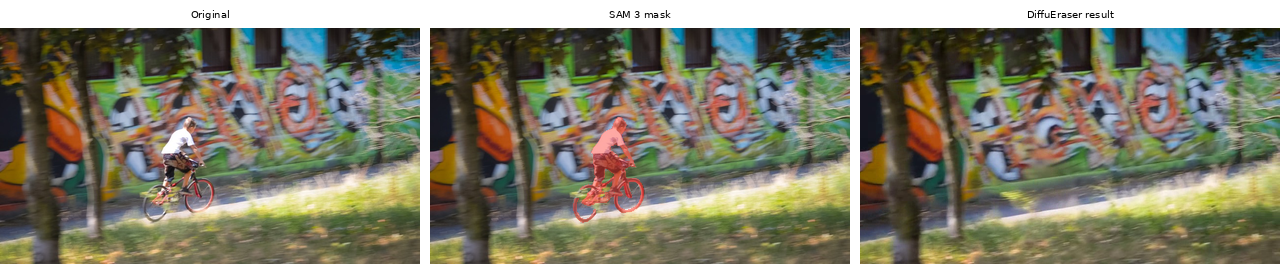
\includegraphics[width=\linewidth]{figures/part3_triptych.png}
\caption{Part 3 triptych on the same bmx-trees frame: original frame, SAM 3 mask, and DiffuEraser result.}
\label{fig:p3-qual}
\end{figure}

\paragraph{Failure analysis.}
The most visible remaining limitation appears when the mask covers a hard background for many frames. Figure~\ref{fig:rhino-failure} shows the rhino sequence, where the occluded grass and body-sized background region remain difficult. DiffuEraser tends to generate a plausible but blurred fill when the true background is never observed for long enough. ROSE can preserve stronger texture locally, but adjacent frames may change appearance, producing background flicker. This suggests that future work should combine generative keyframe repair with explicit temporal consistency losses, flow-guided propagation, or a post-hoc deflickering module.

\begin{figure*}[t]
\centering
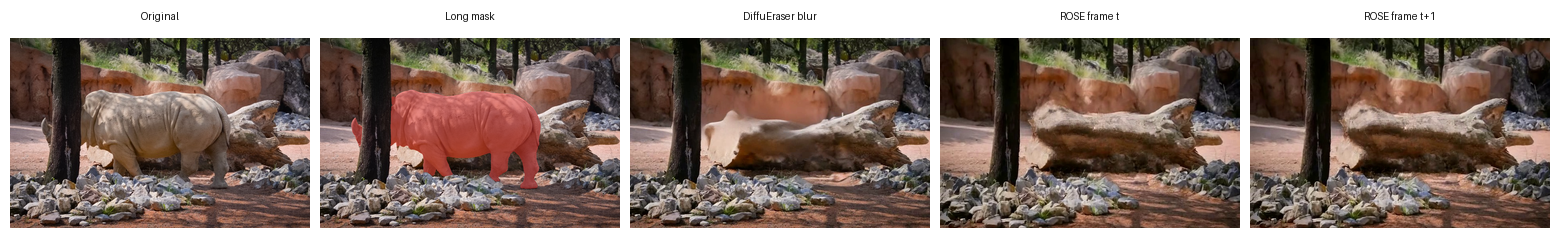
\includegraphics[width=0.95\linewidth]{figures/rhino_failure_strip.png}
\caption{Long-mask failure on rhino. DiffuEraser can blur the generated background, while ROSE may vary between neighboring frames, producing visible flicker in video playback.}
\label{fig:rhino-failure}
\end{figure*}

\section{Conclusion}
The experiments show that video object removal is mask-limited before it is inpainting-limited. The classical Part 1 pipeline is useful for understanding the mechanics of detection, motion filtering, temporal borrowing, and spatial fallback, but it cannot match promptable video segmentation. Part 2 confirms that SAM 2 + ProPainter is a strong practical baseline. Part 3 improves DAVIS mask quality with SAM 3 multi-object initialization and explores generative backends that improve Wild Video perceptual metrics. The main limitation remains long-duration occlusion: when the true background is hidden for many frames, generative methods can blur, and video diffusion methods can flicker. Future work should add mid-sequence re-prompting, uncertainty-aware mask correction, and temporally consistent generative refinement.

\clearpage
{\small
\bibliographystyle{ieeenat_fullname}
\bibliography{main}
}

\end{document}
